\subsection{Análisis Temporal}
Se obtuvo la salida del circuito teniendo a la entrada una señal senoidal de frecuencia 1KHz y de amplitud $0.25 \ \hat{V}$ y otra simulación con la misma entrada pero sumado también ruido blanco con distribución uniforme de amplitud $25 \ m\hat{V}$.
\begin{figure}[H]
	\centering
	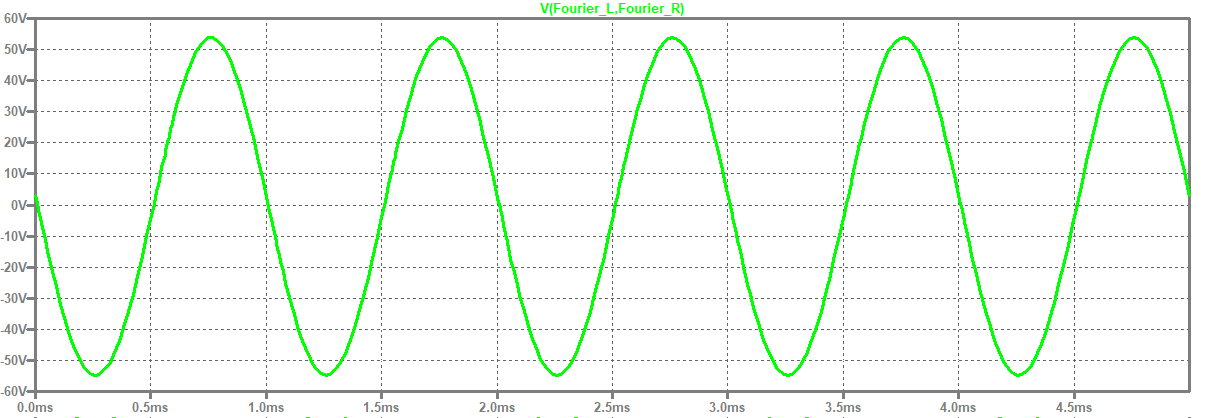
\includegraphics[width=0.8\textwidth]{ImagenesSimulaciones/VRL.png}
		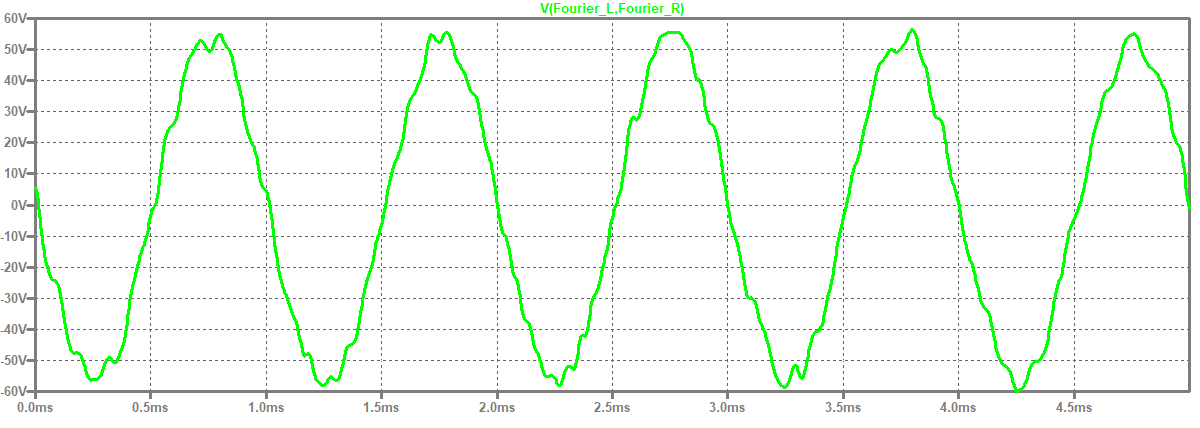
\includegraphics[width=0.8\textwidth]{ImagenesSimulaciones/VRLNoise.png}
	\caption{Tensión sobre la carga con y sin ruido.}
	\label{fig:VRLN}
\end{figure}

\subsection{Análisis en Frecuencia}
Se obtuvo el Bode del sistema como se observa a continuación:
\begin{figure}[H]
	\centering
	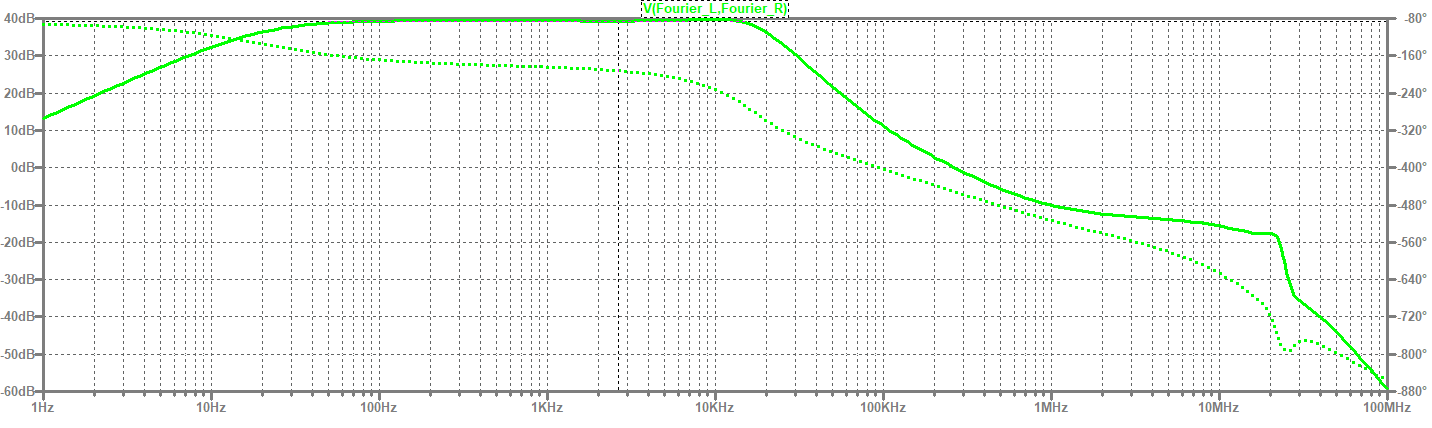
\includegraphics[width=0.9\textwidth]{ImagenesSimulaciones/BODE.png}
	\caption{Bode del sistema.}
	\label{fig:bode}
\end{figure}

Donde se puede apreciar una caida de 3dB respecto a la banda pasante tanto en $20 \ Hz$ como en $20 \ kHz$.

\subsection{Análisis de Impedancias}
Se simuló la impedancia tanto de entrada como de salida.
\begin{figure}[H]
	\centering
	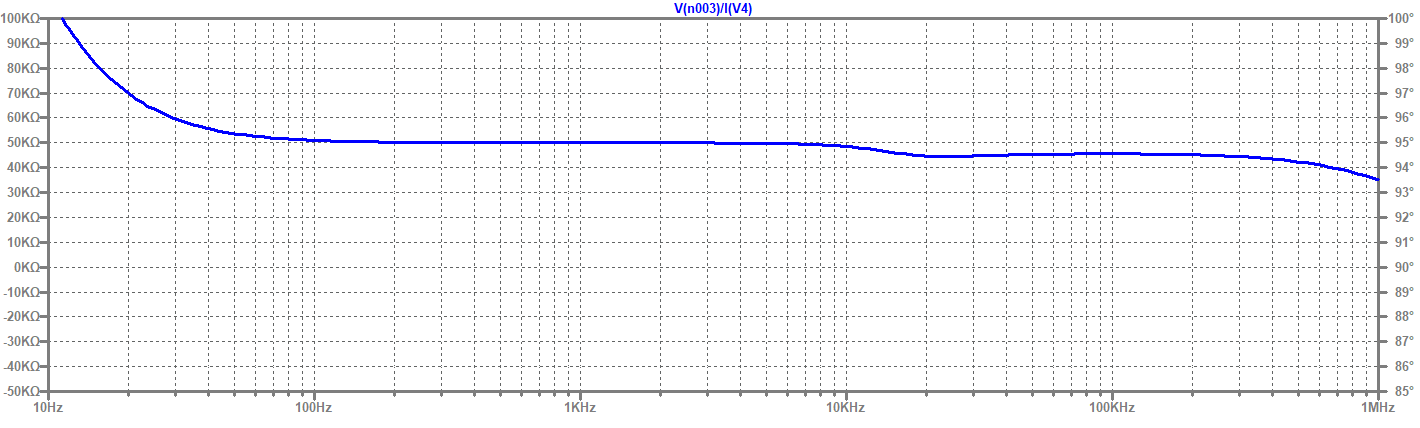
\includegraphics[width=0.9\textwidth]{ImagenesSimulaciones/Zin.png}
	\caption{Impedancia de entrada del sistema.}
	\label{fig:zin}
\end{figure}
Se puede notar que la impedancia de entrada en la banda audible es de $50 \ k\Omega$
\begin{figure}[H]
	\centering
	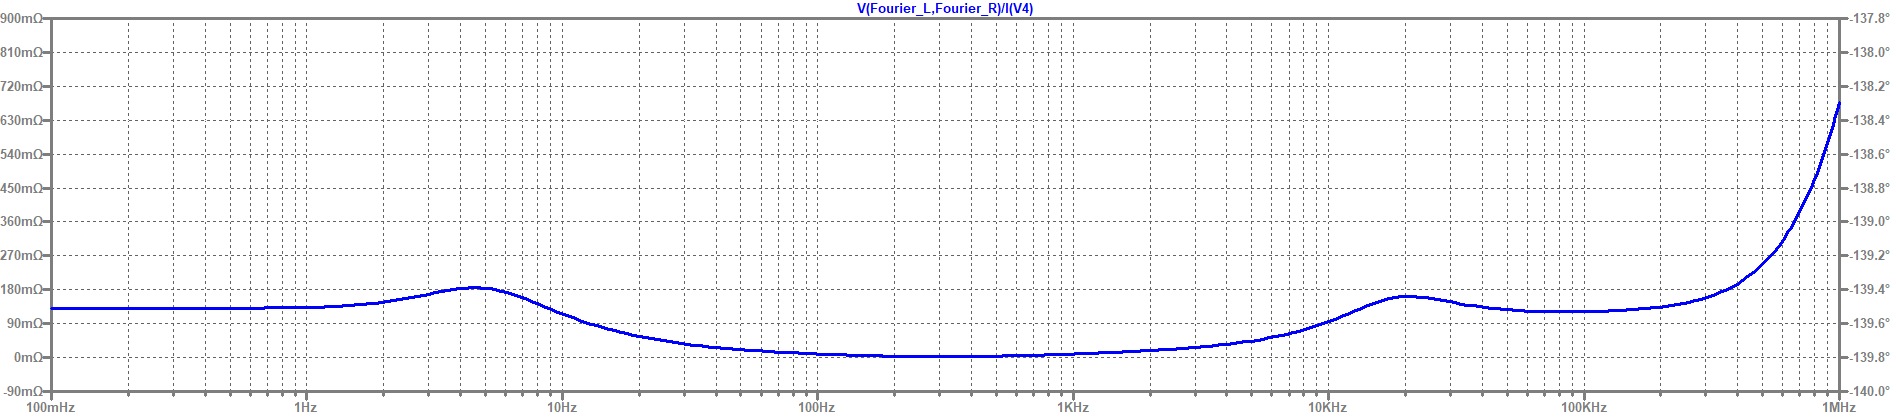
\includegraphics[width=0.9\textwidth]{ImagenesSimulaciones/Zout.png}
	\caption{Impedancia de salida del sistema.}
	\label{fig:zout}
\end{figure}
La impedancia de salida es un valor cercano del orden de las decenas de $m\Omega$, idealmente sería de $8 \ \Omega$ para que haya máxima transferencia de Potencia.
Como también se midió la THD en la simulación obteniendo un valor de $0.400742\%$ cuando se disipa la máxima potencia.

\subsection{Efectos de la resistencia del Jfet}
Dado a que la resistencia del Jfet gobierna la corriente provista por el, variaciones en ella provocan un desvalance tanto en la tensión de salida, agregando un nivel de continua, como la potencia sobre los transistores de salida.

A continuación se muestra una simulación en la cual se puede apreciar el cambio de la tensión de salida provocado por la variación de dicha resistencia.
 \begin{figure}[H]
\centering
	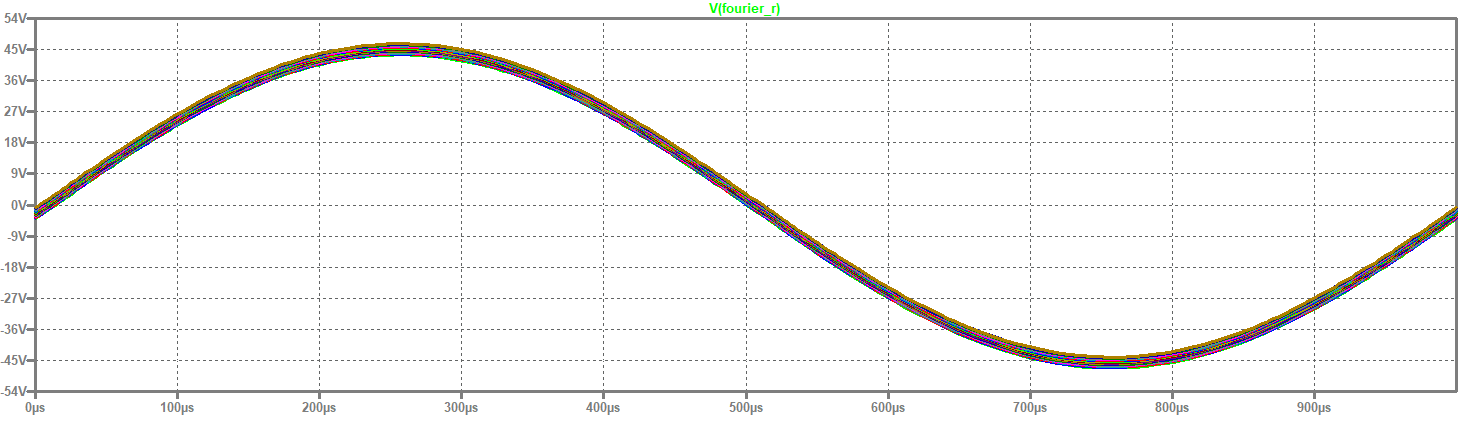
\includegraphics[width=0.7\textwidth]{ImagenesSimulaciones/jfetvar1.png}
	\caption{Variación de la tensión de salida en función de la resistencia del Jfet.}
	\label{fig:mcvl}
\end{figure}

El desvalance en la tensión de salida de cada etapa puede llegar a no ser un problema debido a la configuración de puente H. Teniendo la carga conectada diferencialmente, y al estar en contrafase ambas ramas del circuito, se cancelaría la continua sobre la carga, pero este nivel de continua que carga cada rama resulta un problema debido a que si la potencia disipada por los transistores esta desbalanceada, afecta seriamente al rendimiento.
 \begin{figure}[H]
\centering
	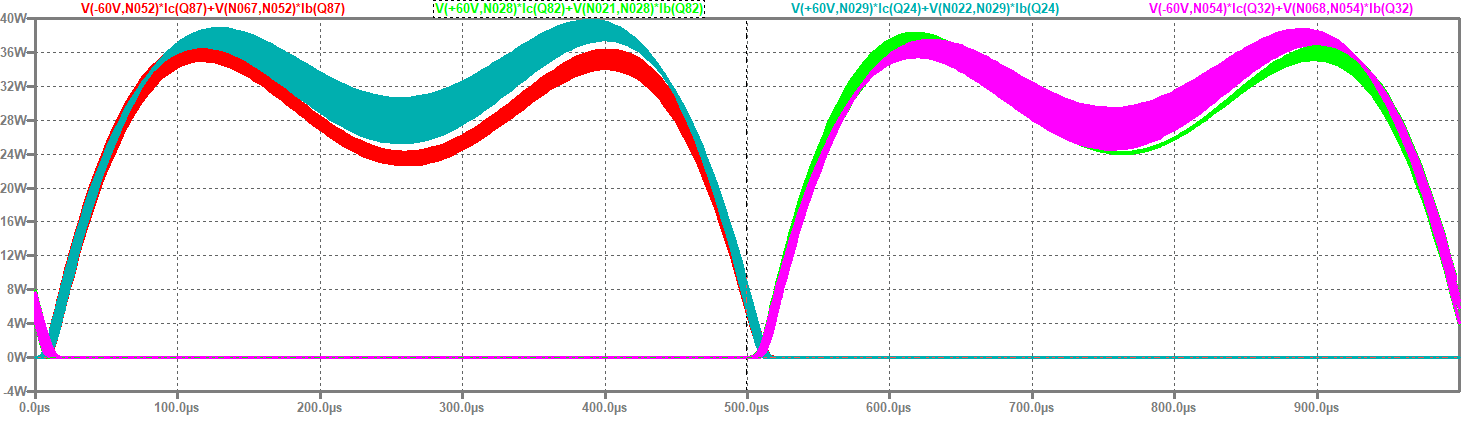
\includegraphics[width=0.7\textwidth]{ImagenesSimulaciones/DesvalanceP.png}
	\caption{Variación de la potencia de los transistores de salida en función de la resistencia del Jfet.}
	\label{fig:mcPl}
\end{figure} 

\subsection{Simulación del rendimiento}
El rendimiento esta definido como:
\begin{align}
\eta = \frac{P_{RL}}{P_{vcc}+P_{vee}}
\end{align}

Para la simulación del rendimiento se utilizaron las siguientes directivas del LTSpice:

\begin{itemize}
\item $.meas Pout AVG V(Fourier_R,Fourier_L)*I(R172)$
\item $.meas Pin AVG -((V(+60V)*I(V2))-(V(-60V)*I(V3)))$
\item $.meas Rend PARAM Pout/Pin$
\end{itemize}

Finalmente, se obtuvo un rendimiento del $0.6977\%$, aproximadamente $70\%$.

\subsection{Análisis de Potencia}
Aquí se muestran las tensiones y potencias relevantes del circuito en cuanto a la elección crítica de componentes.

Comenzando por los emisores comunes la potencia se encuentra cerca del máximo y la tensión $V_{ce}$ en un rango seguro.

\begin{figure}[H]
	\centering
	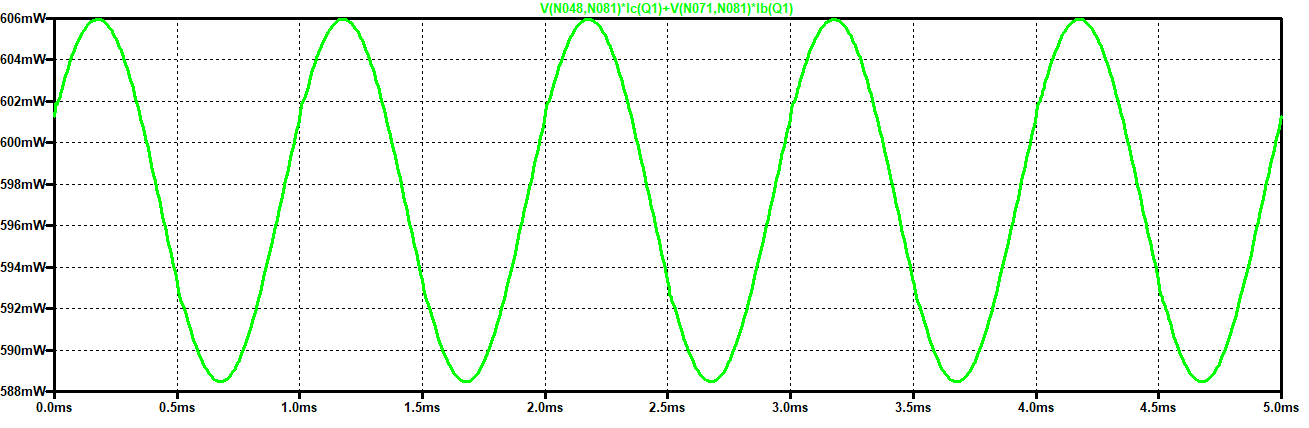
\includegraphics[width=0.8\textwidth]{ImagenesSimulaciones/PEC1.png}
		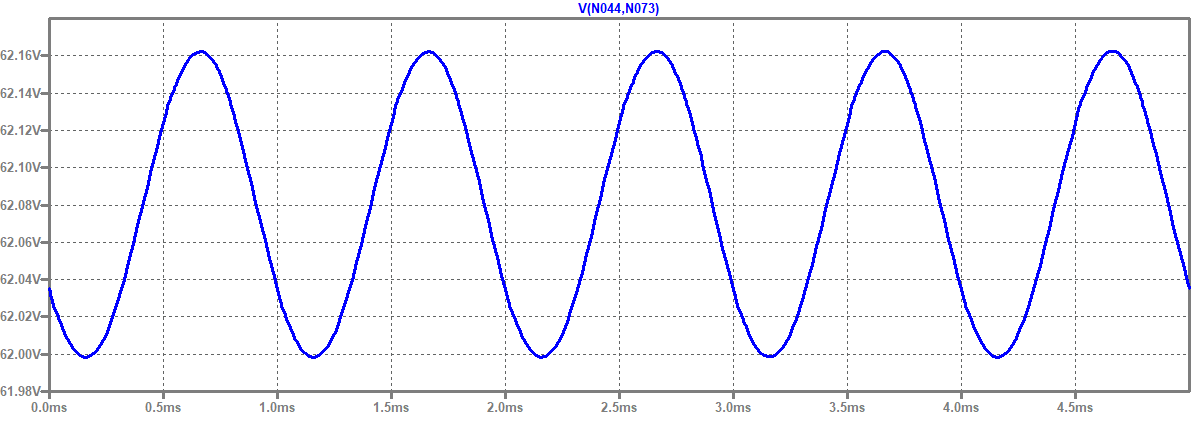
\includegraphics[width=0.8\textwidth]{ImagenesSimulaciones/VEC1.png}
	\caption{Potencia y tensión sobre un emisor común sin carga activa. $546 \ mW$ medios.}
	\label{fig:pec1}
\end{figure}

También se cuenta con que la potencia disipada por las resistencias de colector son cercanas a $0.5 \ W$, por lo que las resistencias a utilizar son de medio Watt. Luego el último emisor común manejará la máxima variación de tensión.

\begin{figure}[H]
	\centering
	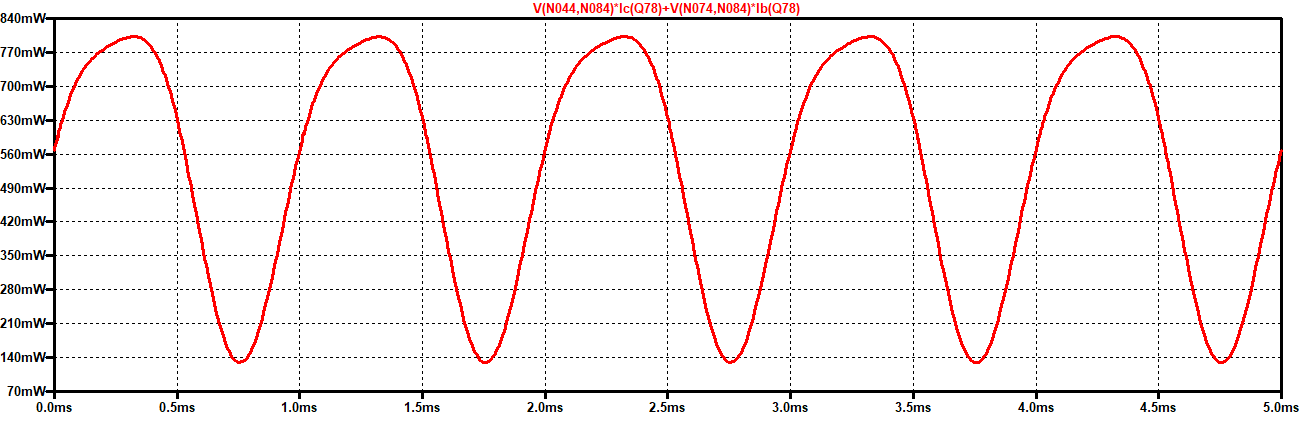
\includegraphics[width=0.8\textwidth]{ImagenesSimulaciones/PECF.png}
		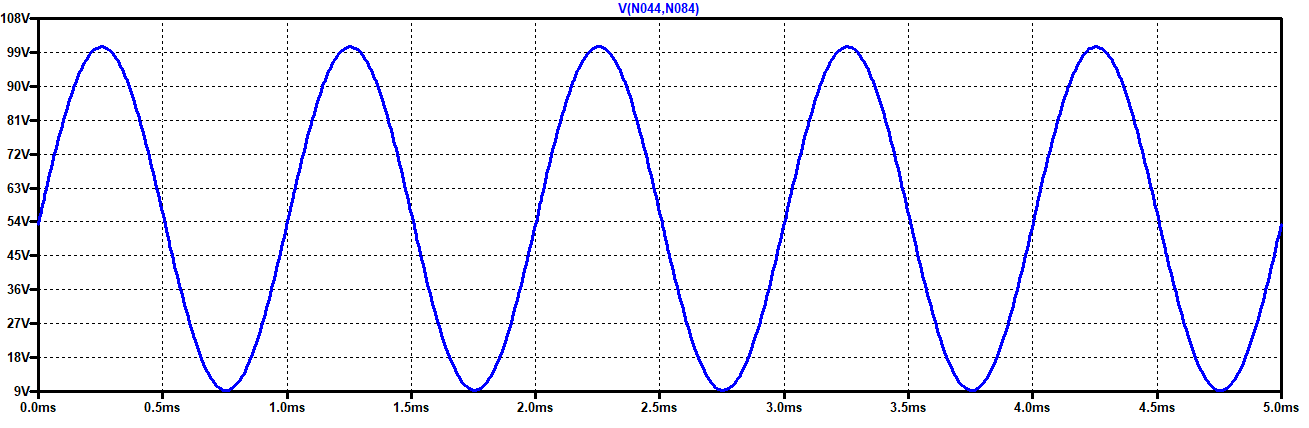
\includegraphics[width=0.8\textwidth]{ImagenesSimulaciones/VECF.png}
	\caption{Potencia y tensión sobre un emisor común con carga activa. $540 \ mW$ medios.}
	\label{fig:pecf}
\end{figure}
%% potencai fuente de corriente de la carga activa
En cuanto a la carga activa, dado que se encuentra en el colector del transistor va a  sufrir también una gran variación de tensión por lo que se necesita un transistor que pueda manejar dicha tensión.
\begin{figure}[H]
	\centering
	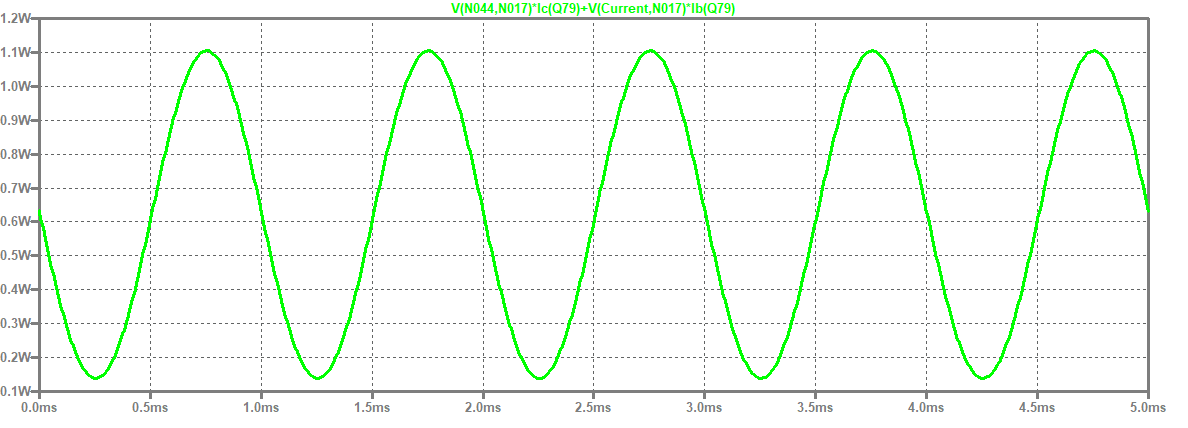
\includegraphics[width=0.8\textwidth]{ImagenesSimulaciones/PCSEC.png}
		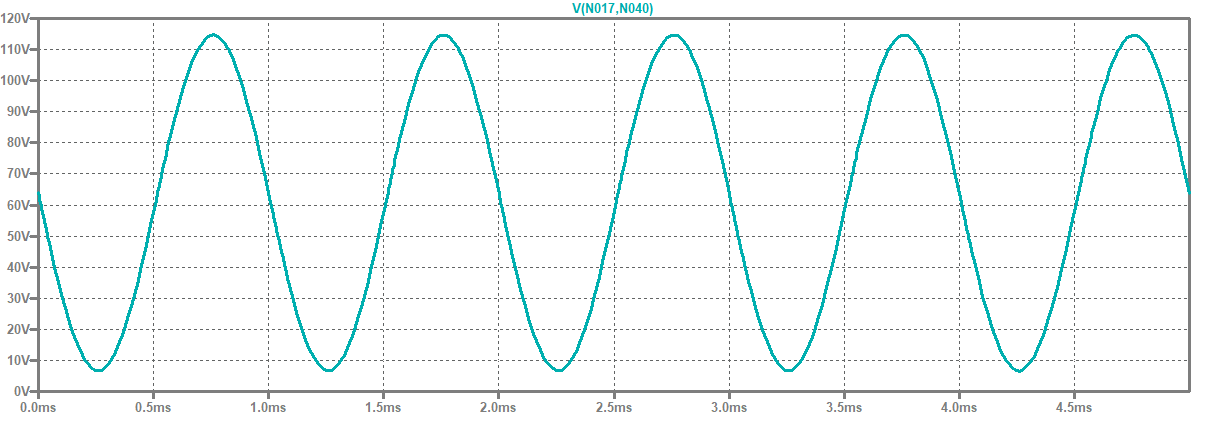
\includegraphics[width=0.8\textwidth]{ImagenesSimulaciones/VCSEC.png}
	\caption{Potencia y tensión sobre la carga activa. $632 \ mW$ media.}
	\label{fig:pcsecf}
\end{figure}

%% potencia de la fuente de corriente del multiplicador de vbe
Continuando por la potencia y tensión correspondiente a la fuente de corriente de la etapa de salida.
\begin{figure}[H]
	\centering
	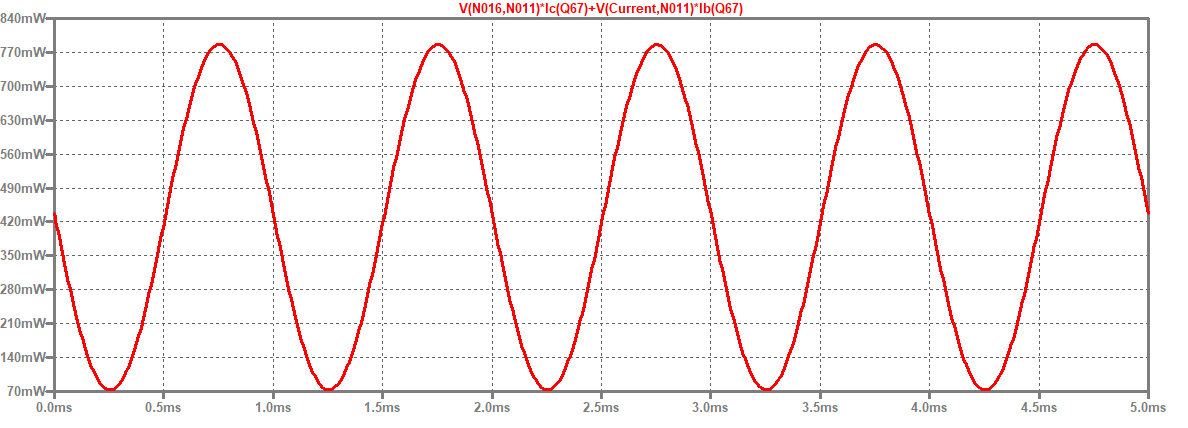
\includegraphics[width=0.8\textwidth]{ImagenesSimulaciones/PCSVBE.png}
		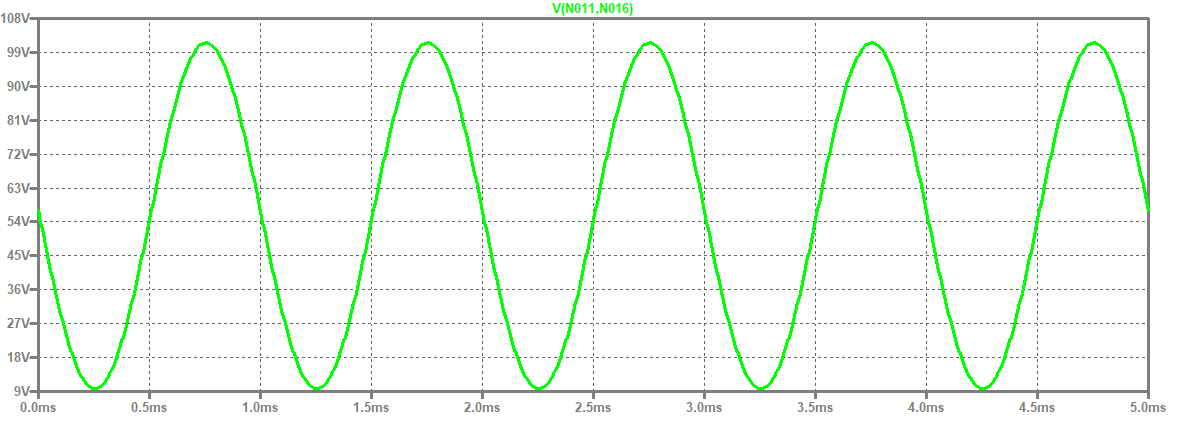
\includegraphics[width=0.8\textwidth]{ImagenesSimulaciones/VCSVBE.png}
	\caption{Potencia y tensión de la fuente de corriente de la salida. $437 \ mW$ medios.}
	\label{fig:pcsvbe}
\end{figure}
%%potencia en el primer transistor de salida
Considerando la potencia de la etapa de salida consideraremos la potencia de las 3 fases, correspondiendo a la primera, la de menor potencia:
\begin{figure}[H]
	\centering
	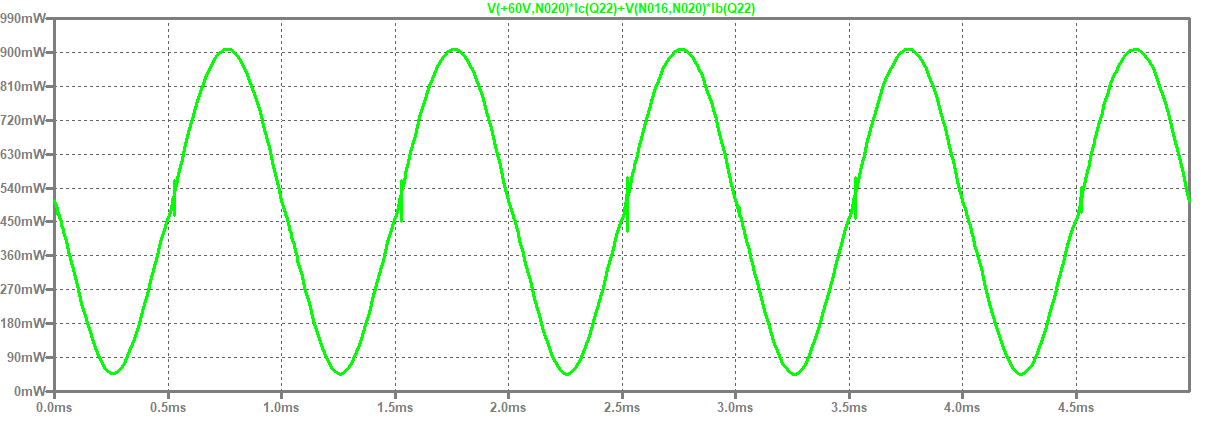
\includegraphics[width=0.8\textwidth]{ImagenesSimulaciones/PO1.png}
		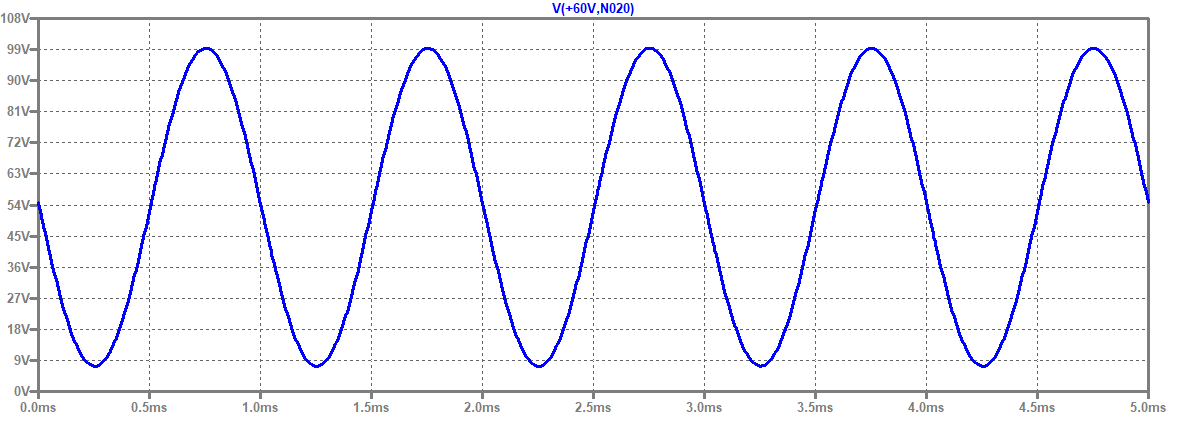
\includegraphics[width=0.8\textwidth]{ImagenesSimulaciones/VO1.png}
	\caption{Potencia y tensión del primer transistor de salida. $488 \ mW$ medios.}
	\label{fig:po1}
\end{figure}
Para el segundo, el cual corresponde a mediana potencia:
\begin{figure}[H]
	\centering
	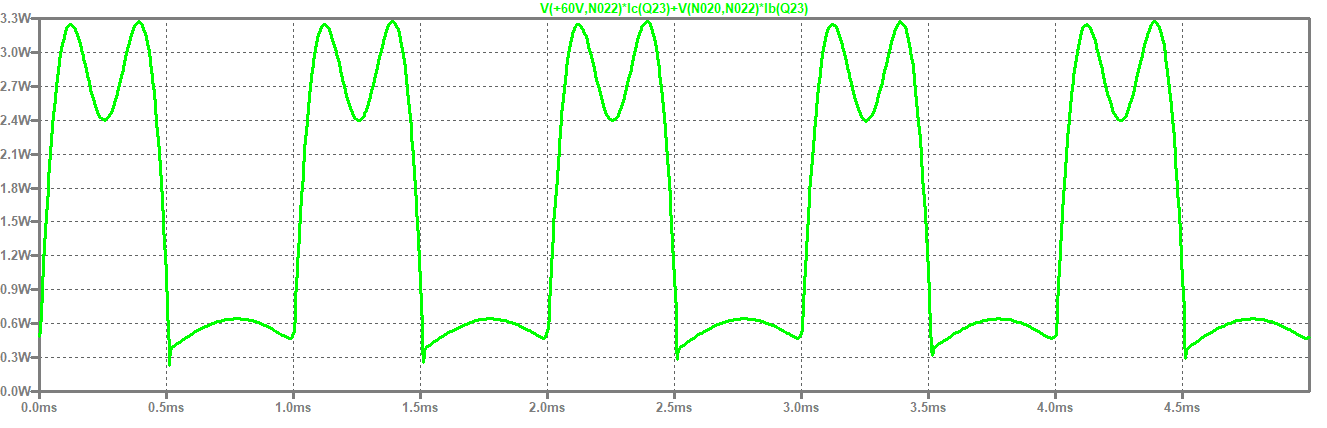
\includegraphics[width=0.8\textwidth]{ImagenesSimulaciones/PO2.png}
		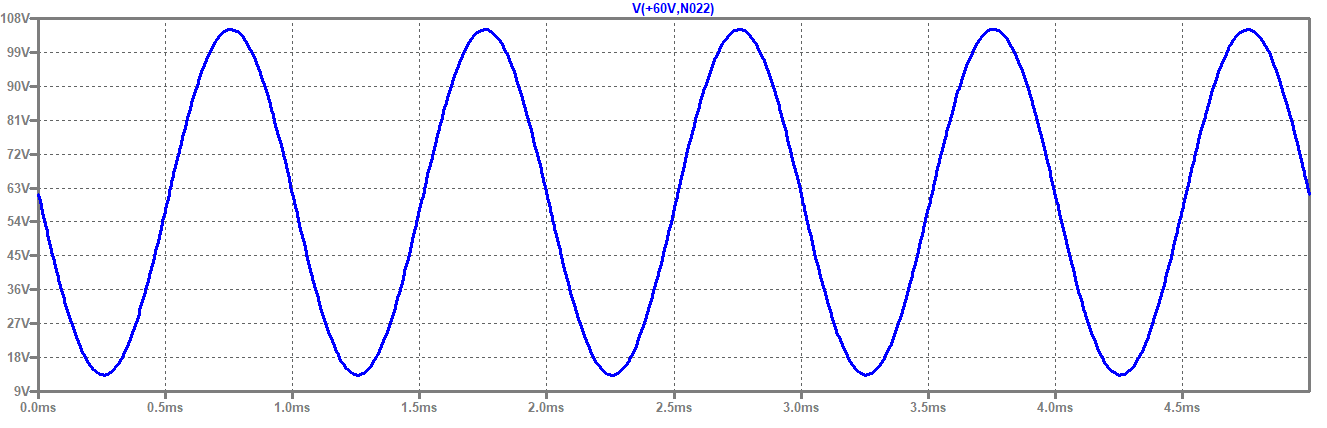
\includegraphics[width=0.8\textwidth]{ImagenesSimulaciones/VO2.png}
	\caption{Potencia y tensión del segundo transistor de salida. $1.411 \ W$ medios.}
	\label{fig:po2}
\end{figure}
Luego para los últimos transistores, los cuales son los que trabajan con la mayor parte de la potencia de salida se obtuvo tanto la potencia como la tensión sobre ellos.
\begin{figure}[H]
	\centering
	\includegraphics[width=0.8\textwidth]{ImagenesSimulaciones/PO3.png}
		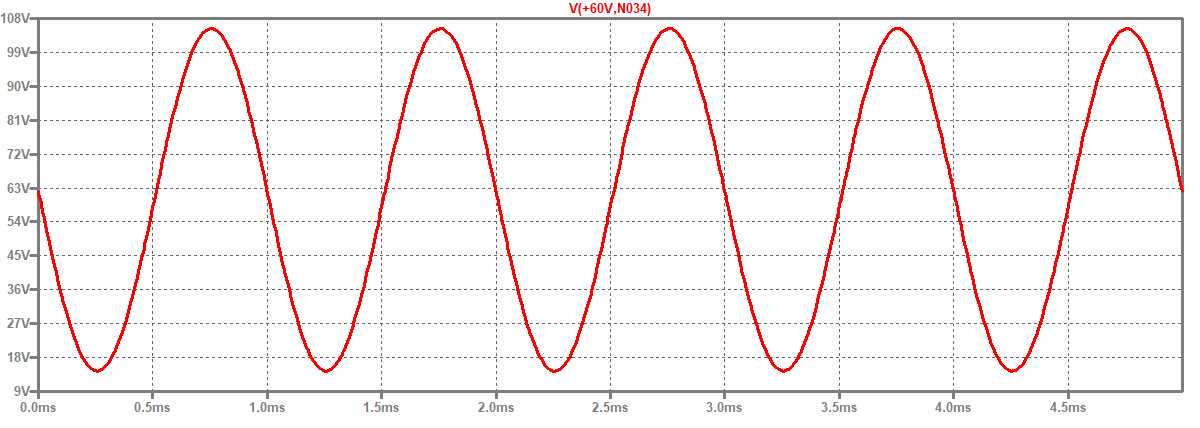
\includegraphics[width=0.8\textwidth]{ImagenesSimulaciones/VO3.png}
	\caption{Potencia y tensión de los transistores de salida. $12.758 \ W$ medios.}
	\label{fig:po3}
\end{figure}
Adicional mente se puede observar que en el gráfico de potencias se dibujo también la potencia del transistor PNP de la rama inferior, para hacer evidente el nivel de simetría que se tiene.

Finalmente se muestra la simulación de potencia sobre la carga.
\begin{figure}[H]
	\centering
	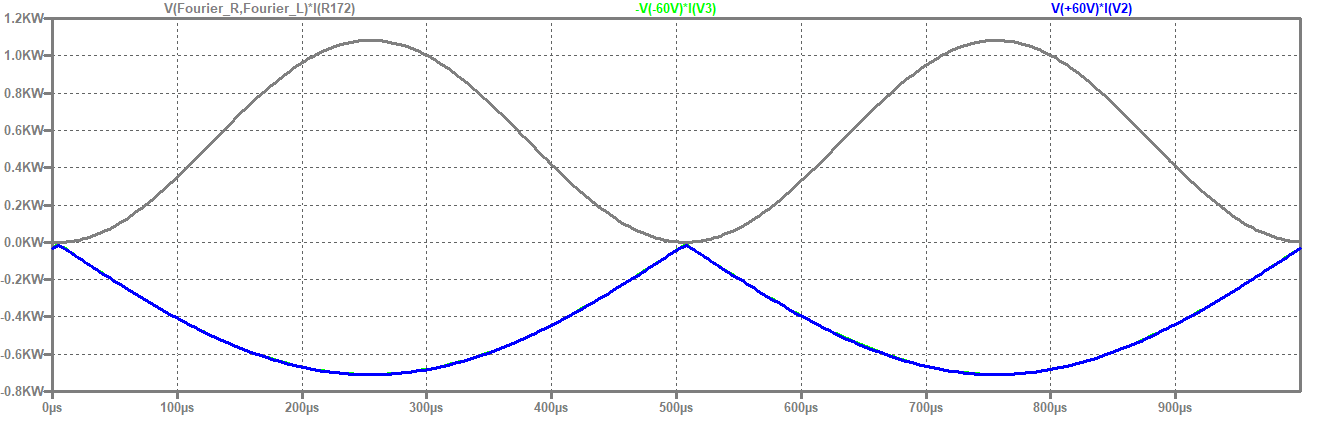
\includegraphics[width=0.8\textwidth]{ImagenesSimulaciones/PRL.png}
	\caption{Potencia sobre la carga. $12.758 \ W$ medios.}
	\label{fig:porl}
\end{figure}
Aquí se pueden apreciar varias cosas. En primer lugar, con una tensión de entrada de $0.5  \ \hat{V}$ se obtiene la mayor potencia, la cual corresponde a aproximadamente $1500 \ W$, también debe notarse que la potencia entregada por la fuente es aproximadamente $0 \ W$ cuando la potencia sobre la carga también lo es.
